\usetikzlibrary{calc}






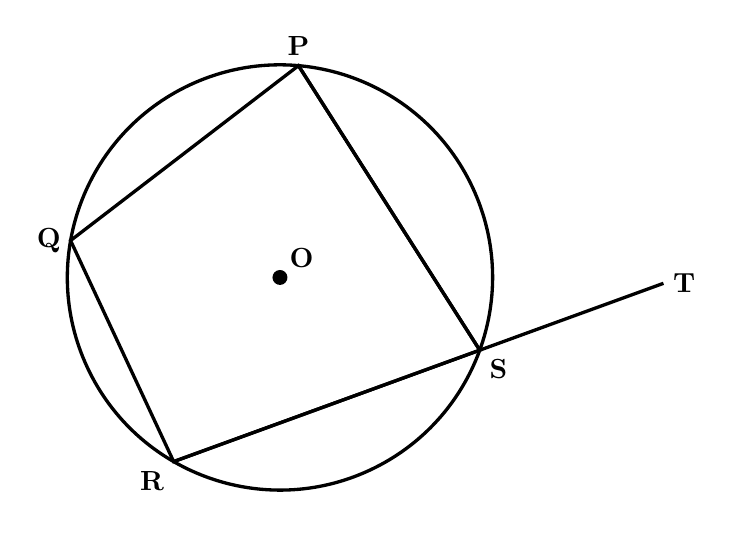
\begin{tikzpicture}[scale=1.8, rotate=25]
    % Define the circle radius
    \def\r{1.5}
    
    % Draw circle
    \draw[very thick] (0,0) circle (\r);
    
    % Define points on the circle for quadrilateral PQRS
    \coordinate (P) at (60:\r);
    \coordinate (Q) at (145:\r);
    \coordinate (R) at (215:\r);
    \coordinate (S) at (315:\r);
    
    % Draw quadrilateral PQRS
    \draw[very thick] (P) -- (Q) -- (R) -- (S) -- cycle;
    
    % Draw diagonal PS
    \draw[very thick] (P) -- (S);
    
    % External point T on the extended line from R through S
    \coordinate (T) at ($(R)!1.6!(S)$);
    \draw[very thick] (R) -- (T);
    
    % Center point O with dot
    \fill (0,0) circle (1.5pt);
    
    % Labels with bold font (counter-rotated so text is horizontal)
    \node[above, font=\bfseries] at (P) {P};
    \node[left, font=\bfseries] at (Q) {Q};
    \node[below left, font=\bfseries] at (R) {R};
    \node[below right, font=\bfseries] at (S) {S};
    \node[right, font=\bfseries] at (T) {T};
    \node[above right, font=\bfseries] at (0,0) {O};
\end{tikzpicture}